\documentclass[../../main.tex]{subfiles}

\begin{document}

At the time the Wedge paper was published, ciphers that offer forward
secrecy were not common place; hence, the authors of Wedge deemed it
unnecessary to provide support for this category of ciphers. However,
forward secrecy has gained popularity since, with
[STATISTIC][CITATION]. We have, therefore, designed our system to
accomodate ciphers within this category. As of TLSv1.2 ciphers that
offer forward secrecy employ some variant of Diffie-Hellman (DH) Key
Exchange to establish the \texttt{PremasterSecret}. Before discussing
the SSL/TLS handsake for these ciphers, we provide a brief
explaination of DH Key Exchange.


DH Key Exchange is an asymmetric cryptographic algorithm used to
arrive at a shared secret between two parties. DH Key Exchange can be
best illustrated using the famous ``paint mixing'' analogy. The
analogy is presented in Figure~\ref{fig:paint}.
\begin{enumerate}
  \item The partiticpants agree to using a publicly known ``paint
    color''
  \item Each participant generates a secret ``paint color''
  \item Each participant ``mixes'' their ``secret color'' with the
    ``public color'' they previously agreed to use
  \item The participants \textit{exchange} the ``paint mixtures'' from
    the previous step
  \item The participants combine the ``paint mixture'' they received
    with their own ``secret paint''. Both parties now possess the same
    ``shared secret paint''.
\end{enumerate}
The security of DH Key Exchange relies on the assumption that it is
computationally difficult to seperate the ``paint mixtures''.
\begin{figure}[H]
  \centering
  
  \caption{DH Key Exchange paint analogy}
  \label{fig:paint}
\end{figure}
Moreover, by creating new ``secret paints'' for each session and
purging all the ``paints'' from memory after a session is complete,
one obtains Ephemeral DH Key Exchange (DHE). DHE offers forward
secrecy because no long-term private secret is used to negotiate the
shared secret; hence, compromising a single session's ``secret
paints'' does not affect any other session (new ``secret paints'' are
used for new sessions).

For our project, we concentrated on Elliptical Curves DHE (ECDHE).
This is a variant of DHE that utilises Elliptical Curves to ``mix''
the ``paints''. The mathematics behind ECDHE is beyond the scope of
this report, but the interested reader may refer to [CITATION] for
further details. The steps in the SSL/TLS handshake when using an
ECDHE cipher (``ECDHE handshake'') are presented in
Figure~\ref{fig:ecdhe-pristine}.

\begin{figure}[H]
  \centering
  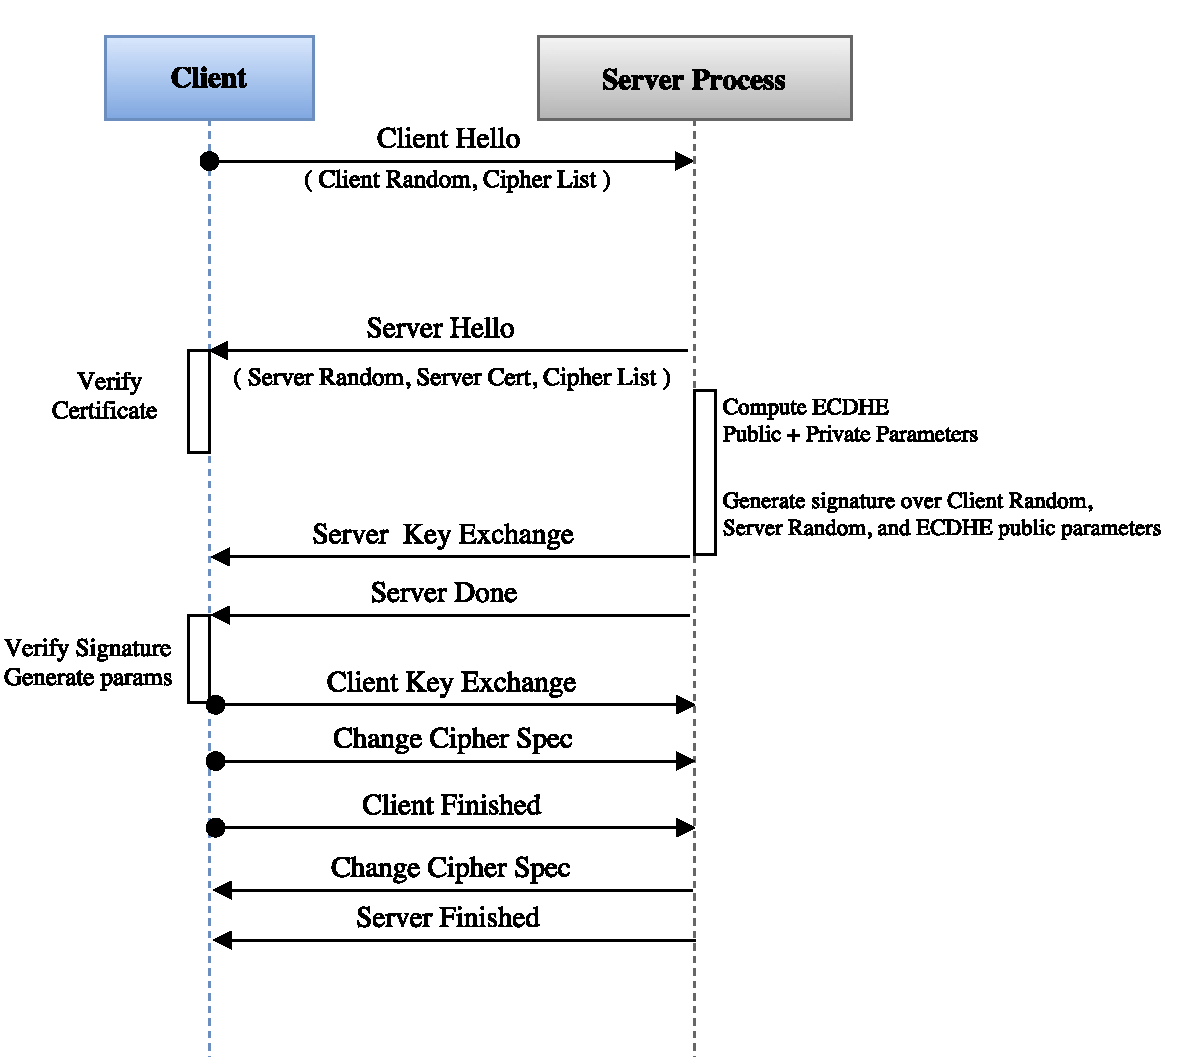
\includegraphics[scale=0.4]{images/EC-DHE-Handshake-pristine.pdf}
  \caption[``ECDHE handshake'']{SSL/TLS handshake when using an ECDHE
    cipher}
  \label{fig:ecdhe-pristine}
\end{figure}

Similair to the ``RSA handshake'', the ``ECDHE handshake'' begins by
establishing the values for \crandom~and \srandom. In performing this
exchange, the involved parties also agree on the Elliptic Curve
(``well-known paint'') to be used in negotiating the shared secret.
Following that, the server computes its private parameter (``secret
paint'') and the corresponding public parameter (``paint mixture''). A
hash function is applied across the public parameter, \srandom, and
\crandom. This resulting message digest is signed using the long-term
private key and is sent to the client, attached to the public
parameter. The digital signature is computed to:
%This can be phrased better, leaving it for now.
\begin{itemize}
  \item Prove the identity of the server to the client
  \item Prove that the ECDHE public parameter received was indeed
    computed by the server, preventing man in the middle attacks. 
\end{itemize}
The client verifies the signature received, computes their own private
and public parameters, and sends the public parameter to the server.
The client and server may now derive the \texttt{PremasterSecret},
\texttt{MasterSecret}, and the session key block. The handshake then
proceeds in the same way as the ``RSA handshake''.

Clearly, from the discussion above, the long-term private key is used
only for verification purposes in the ``ECDHE handshake''. To secure
the long-term secret, one may elect to provide an interface that
receives \crandom, \srandom, and ECDHE public parameter, computes the
message digest, and derives the signature. However, such an interface
allows an adversary to \textit{influence} key generation, if they
explot the untrusted component. Instead, we created an interface that
accepts \crandom~ and returns the signature. The values of~\srandom~,
the private parameter, and the public parameter are computed in the
enclave. This provides the same freshness property described earlier
in the context of the ``RSA handshake'', preventing the attacker from
acquiring any useful information by exploiting the interface. The
resulting interface is depicted in Figure~\ref{fig:ecdhe-handshake}.

\begin{figure}[H]
  \centering
  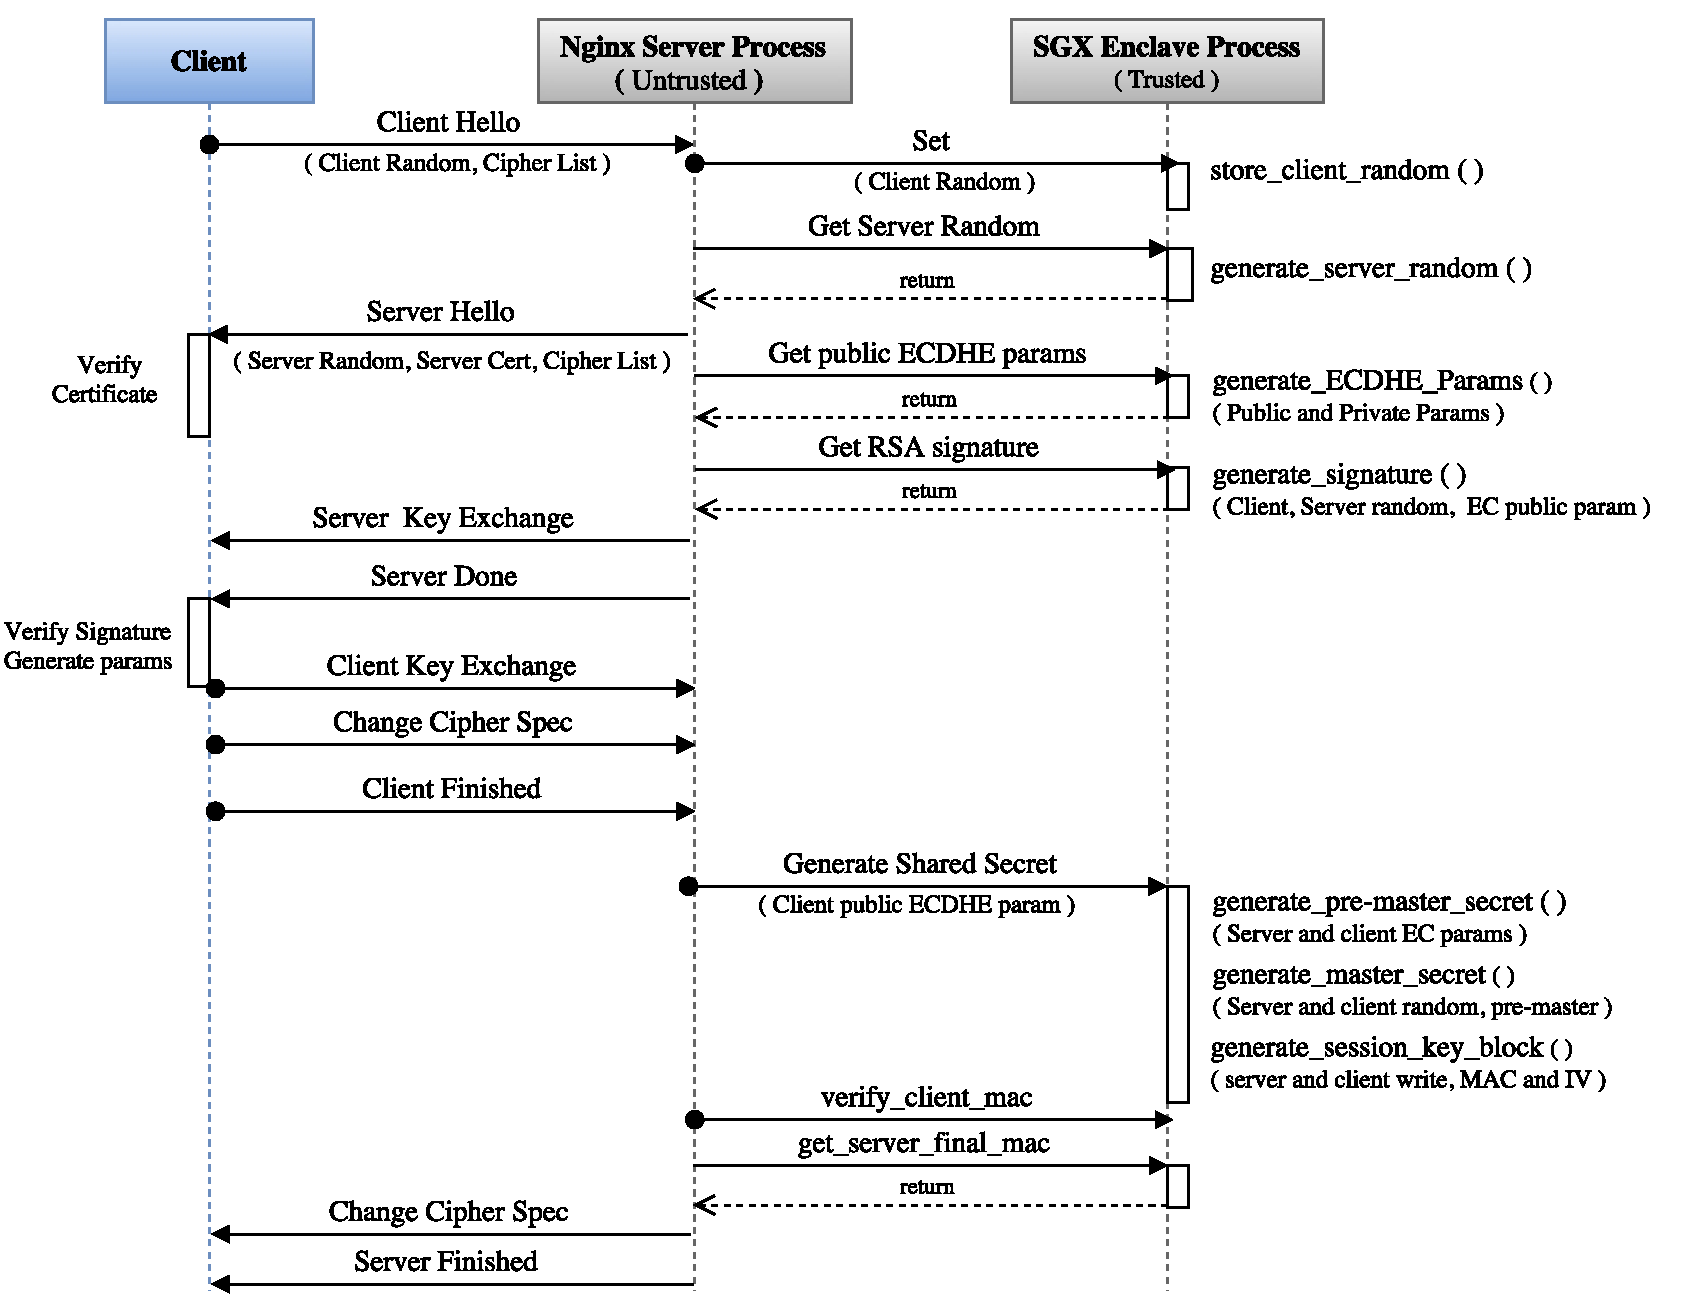
\includegraphics[scale=0.4]{EC-DHE-Handshake.pdf}
  \caption{``ECDHE Handshake'' with long-term private key in an SGX
    enclave}
  \label{fig:ecdhe-handshake}
\end{figure}

\end{document}

%%% Local Variables:
%%% mode: latex
%%% TeX-master: "../../main"
%%% End:
